\appendix
\renewcommand{\thesection}{\Alph{section}}
\renewcommand\thefigure{\thesection.\arabic{figure}}
\renewcommand\thelisting{\thesection.\arabic{listing}} 
\addchap{Anhang}

\section{Ausgaben zur Kompilierung eines Programms mit LLVM-Tools}

\begin{code}
\inputminted[linenos]{llvm}{../Resources/Code/c-to-llvm/main.ll}
\caption{Kompletter LLVM-IR-Code nach Kompilierung aus C-Source}
\label{lst:llvm-von-c}
\end{code}

\newpage

\begin{code}
\inputminted[linenos]{nasm}{../Resources/Code/c-to-llvm/main.s}
\caption{Assemblercode nach Kompilierung aus LLVM-IR}
\label{lst:assembler-von-llvm}
\end{code}

\newpage

\section{Beispiele zur Visualisierung von Listing \ref{lst:llvm-compare-main-cpp}}
\label{sec:beispiele-zur-visualisierung}

\begin{figure}[H]
\centering
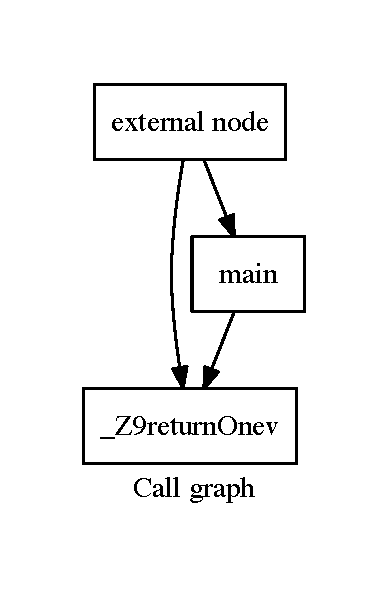
\includegraphics[scale=.8]{../Resources/Bilder/main_callgraph.pdf}
\caption{Call-Graph von \texttt{main.ll}}
\label{fig:main-callgraph}
\end{figure}

\begin{figure}[H]
\begin{minipage}{.4\textwidth}
\centering
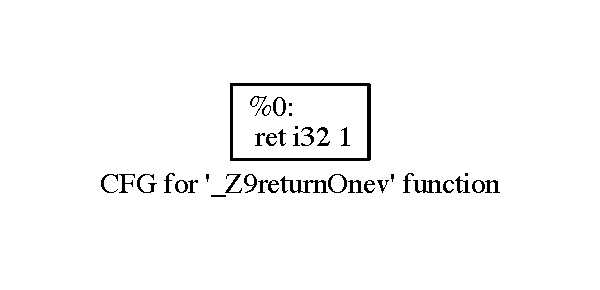
\includegraphics[scale=.8,page=1]{../Resources/Bilder/main_cfg.pdf}
\end{minipage}
\begin{minipage}{.5\textwidth}
\centering
\includegraphics[scale=.8,page=2]{../Resources/Bilder/main_cfg.pdf}
\end{minipage}
\caption{Controlflow-Graphen von \texttt{main.ll}}
\label{fig:main-cfg}
\end{figure}

\begin{figure}[H]
\centering
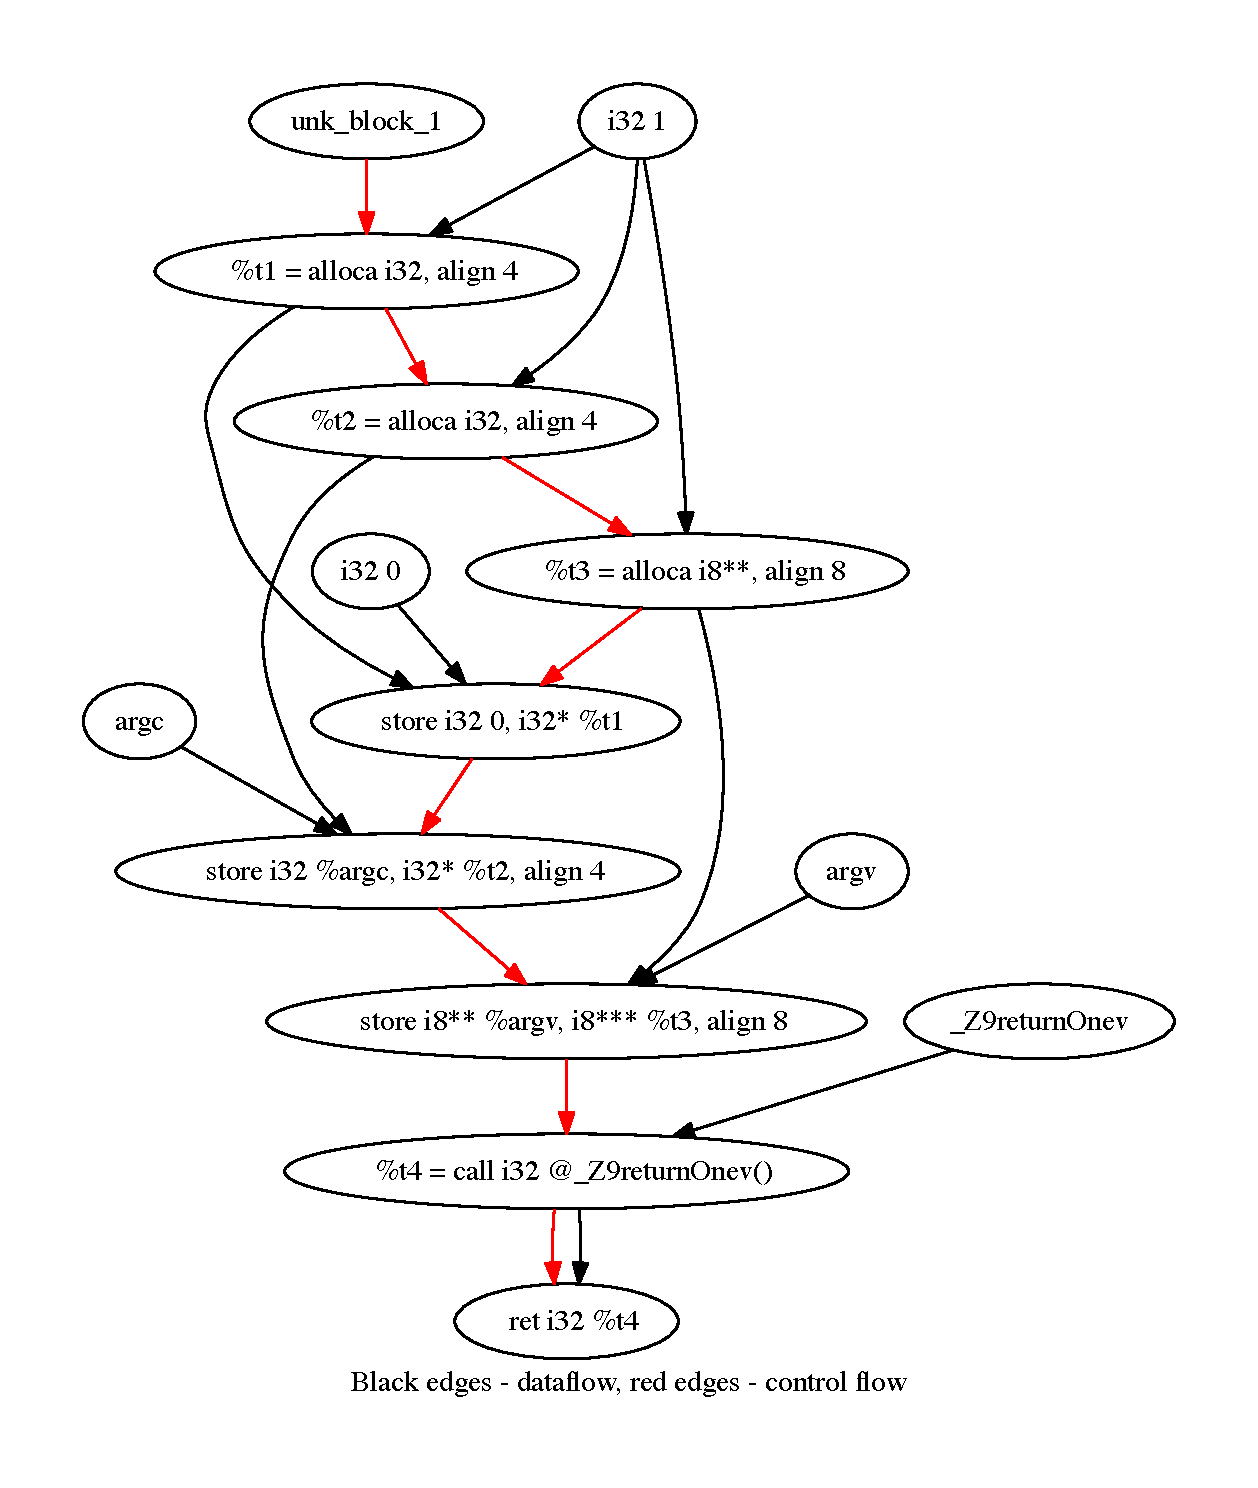
\includegraphics{../Resources/Bilder/cfg_dfg.pdf}
\caption{\gls{CFG-DFG} von \texttt{main.ll}}
\label{fig:main-cfg-dfg}
\end{figure}

\newpage

\section{Generierter LLVM-IR-Code von \textit{Dagger}}
Der folgende \gls{LLVM}-\gls{IR}-Code wurde aus der kompilierten Datei \texttt{main.out} aus Abschnitt \ref{entwicklung-eines-beispiel-programms-und-kompilierung-mit-llvm} mit dem Programm \texttt{llvm-dec} aus dem Projekt \textit{Dagger} gemäß Listing \ref{lst:llvm-dec-dagger} generiert.

\begin{code}
\begin{minted}[linenos]{bash}
~/Developer/dagger/build/bin/llvm-dec main.out -o main.dagger.ll
\end{minted}
\caption{Befehl zur Dekompilierung mit \textit{Dagger}}
\label{lst:llvm-dec-dagger}
\end{code}

\begin{code}
\inputminted[linenos]{llvm}{../Resources/Code/c-to-llvm/dagger/main.dagger.ll}
\caption{Generierter LLVM-IR-Code von Dagger}
\label{lst:llvm-von-obj-mit-dagger}
\end{code}

\newpage

\section{Installation von LLVM, Clang und Fracture unter Mac OSX}
\label{sec:installation-von-llvm-clang-und-fracture-unter-mac-osx}

\begin{code}
\begin{minted}[linenos]{bash}
# Installation der XCode command-line-tools
xcode-select --install
# Installation von autoconf und automake
brew install autoconf automake
# Setzen des Installationspfades
export DESTINATION=$HOME/Developer
# Installation von LLVM und Clang
cd $DESTINATION
git clone https://github.com/draperlaboratory/llvm llvm
cd llvm/tools
git clone https://github.com/draperlaboratory/clang clang
cd ..
./configure --enable-debug-symbols --prefix=/usr/local \
    --build=x86_64-apple-darwin13.3.0
make -j16
sudo make install
# Installation von Fracture
cd $DESTINATION
git clone https://github.com/draperlaboratory/fracture.git fracture
cd fracture
export CXXFLAGS="-std=c++11 -stdlib=libc++ \
    -I/Applications/Xcode.app/Contents/Developer\
    /Toolchains/XcodeDefault.xctoolchain/usr/lib/c++/v1"
./autoconf/AutoRegen.sh
./configure --enable-debug-symbols --with-llvmsrc=$DESTINATION/llvm/ \
    --with-llvmobj=$DESTINATION/llvm/
make -j16
\end{minted}
\caption{Kompilieren von Fracture}
\label{lst:kompilieren-von-fracture}
\end{code}

\newpage

\section{Die Erstellung eines CMake-Projekts am Beispiel von binSpector}
\label{sec:die_erstellung_eines_cmake_projekts_am_beispiel_von_binspector}

\begin{code}
    \inputminted[linenos]{cmake}{/Users/michaelriedel/Developer/binSpector/docs/CMakeLists.txt}
    \caption{Die Datei \texttt{binSpector/docs/CMakeLists.txt}}
    \label{lst:binspector_docs_cmakelists_txt}
\end{code}

\begin{code}
    \inputminted[linenos]{cmake}{/Users/michaelriedel/Developer/binSpector/lib/CMakeLists.txt}
    \caption{Die Datei \texttt{binSpector/lib/CMakeLists.txt}}
    \label{lst:binspector_lib_cmakelists_txt}
\end{code}

\newpage

\begin{code}
	\inputminted[linenos]{cmake}{/Users/michaelriedel/Developer/binSpector/tools/binSpector/CMakeLists.txt}
    \caption{Die Datei \texttt{binSpector/tools/binSpector/CMakeLists.txt}}
    \label{lst:binspector_tools_cmakelists_txt}
\end{code}